% Poster Template for the Okinawa Institute of Science and Technology (OIST)
% Created by Jeremie Gillet on June 2019

\documentclass[
    a0paper, % Size of poster
    landscape, % Orientation
    fontscale=0.34 % General scaling for fonts, increase the number for smaller fonts (considered removing text first)
    ]{baposter}
    
% Graphics
\usepackage{graphicx} % Required for including images
\graphicspath{{figures/}} % Directory in which figures are stored

% Add any packages you need here
\usepackage{amsmath} % For typesetting math
\usepackage{lipsum}  % For dummy text

% Set up how figure and table captions are displayed
\usepackage{caption}
\captionsetup{
  font=footnotesize,% set font size to footnotesize
  labelfont=bf % bold label (e.g., Figure 3.2) font
}

\newcommand{\beq}{\begin{equation}}
\newcommand{\eeq}{\end{equation}}
\newcommand{\beqs}{\begin{equation*}}
\newcommand{\eeqs}{\end{equation*}}
\newcommand{\of}[1]{\left(#1\right)}

% Defining colors
\selectcolormodel{HTML}
\definecolor{OIST}{HTML}{C80019} 
\definecolor{DarkRed}{RGB}{100,0,10}

% Changing fonts family
\renewcommand{\familydefault}{\sfdefault}
\usepackage{helvet}

% Starting document, feel free to change the style of headers and boxes
% Documentation can be found here: http://www.brian-amberg.de/uni/poster/
% Unfortunately it is not very complete
\begin{document}
\begin{poster}{ % General poster options
    columns=6, % Number of columns, maximum 6
    eyecatcher=true, % Set to false for ignoring the left logo in the title and move the title left
    background=none, % No background
    linewidth=1pt, % Width of the border lines around content boxes
    textborder=rectangle, % Format of the border around content boxes, can be: none, bars, coils, triangles, rectangle, rounded, roundedsmall, roundedright or faded
    borderColor=OIST, % Border color
    headerheight=0.13 \textheight, % Height of the header
    headershape=rectangle, % Specify the rounded corner in the content box headers, can be: rectangle, small-rounded, roundedright, roundedleft or rounded
    headerfont=\large \sf \bf, % Large, bold and sans serif font in the headers of content boxes
    headerborder=closed, % Adds a border around the header of content boxes
    headershade=plain, % Single color in the background
    headerColorOne=white, % Background color for the header in the content boxes
    headerFontColor=DarkRed, % Text color for the header text in the content boxes
    boxColorOne=white, % Background color of the content boxes
} 
{ 
\includegraphics[height=.75 \headerheight]{logo.jpg} } % Eyecatcher on the left
{ \color{OIST}\huge Stenotic Channel Flow using the Lattice Boltzmann Method } % Poster title
{ \color{OIST}\small
  \vspace{1em} 
  Alexandru Mihai\\
  alexandru.mihai@oist.jp\\
  Okinawa Institute of Science and Technology
} % Authors
{ 
\includegraphics[height=.75 \headerheight]{logo.jpg} } % Eyecatcher on the right


\begin{posterbox}[name=intro,column=0,span=2, row=0]{Abstract}
The Lattice Boltzmann Method provides an accessible avenue to analyze and model complex fluid dynamics. We analyze the flow through a constricted channel in two dimensions using the LBGK collision model. There are currently no analytic solutions known for the flow through such a geometry. We investigated the transition period of Reynolds numbers where the flow is neither laminar nor turbulent as well as the boundary conditions necessary to produce a stable simulation. Initial results show that this transition period occurs for Reynolds numbers of approximately 1000 to 1500 and that velocity boundaries produce less numerical aberrations. Simulations were also conducted with the open source library OpenLB. Two dimensional as well as three dimensional results using the turbulent Smagorinski Turbulent Model were analyzed.
\end{posterbox}


\begin{posterbox}[name=def,column=0,span=2, below=intro]{The Boltzmann Transport Equation}
\beq \frac{\partial f\of{x,\vec{u},t}}{\partial t} + \vec{u}\cdot \nabla f\of{x,\vec{u},t} = \Omega \eeq
where $f\of{x,\vec{u},t}$ is the particle distribution function, $\vec{u}$ is the particle velocity, and $\Omega$ is the collision operator. We also know that collisions of particles tend to relax the particle distribution function. Thus we have that 
\beqs \Omega = \frac{-1}{\tau}\left[ f\of{x,\vec{u},t} - f^{eq}\of{x,\vec{u},t}\right] \eeqs
where $\tau$ is the relaxation time and $f^{eq}$ is the equilibrium distribution function. The equilibrium distribution is derived from the solution of the Maxwell Equations and the conservation of energy and momentum laws. From this we see that our continuous time equation is 
\beqs  \frac{\partial f\of{x,\vec{u},t}}{\partial t} + \vec{u}\cdot \nabla f\of{x,\vec{u},t} = -\frac{1}{\tau}\left[ f\of{x,\vec{u},t} - f^{eq}\of{x,\vec{u},t}\right] \eeqs
Following a simple space and time discretization the explicit Lattice Boltzmann Equation is found:
\beq f_i\of{x+e_i \Delta t, t + \Delta t} + f_i\of{x,t} = \frac{-\left[ f_i\of{x,t} - f_i^{eq}\of{x,t}\right] }{\tau}\eeq
\end{posterbox}


\begin{posterbox}[name=distribution,column=0,span=2, below=def]{The Particle Distribution Function}
\centering
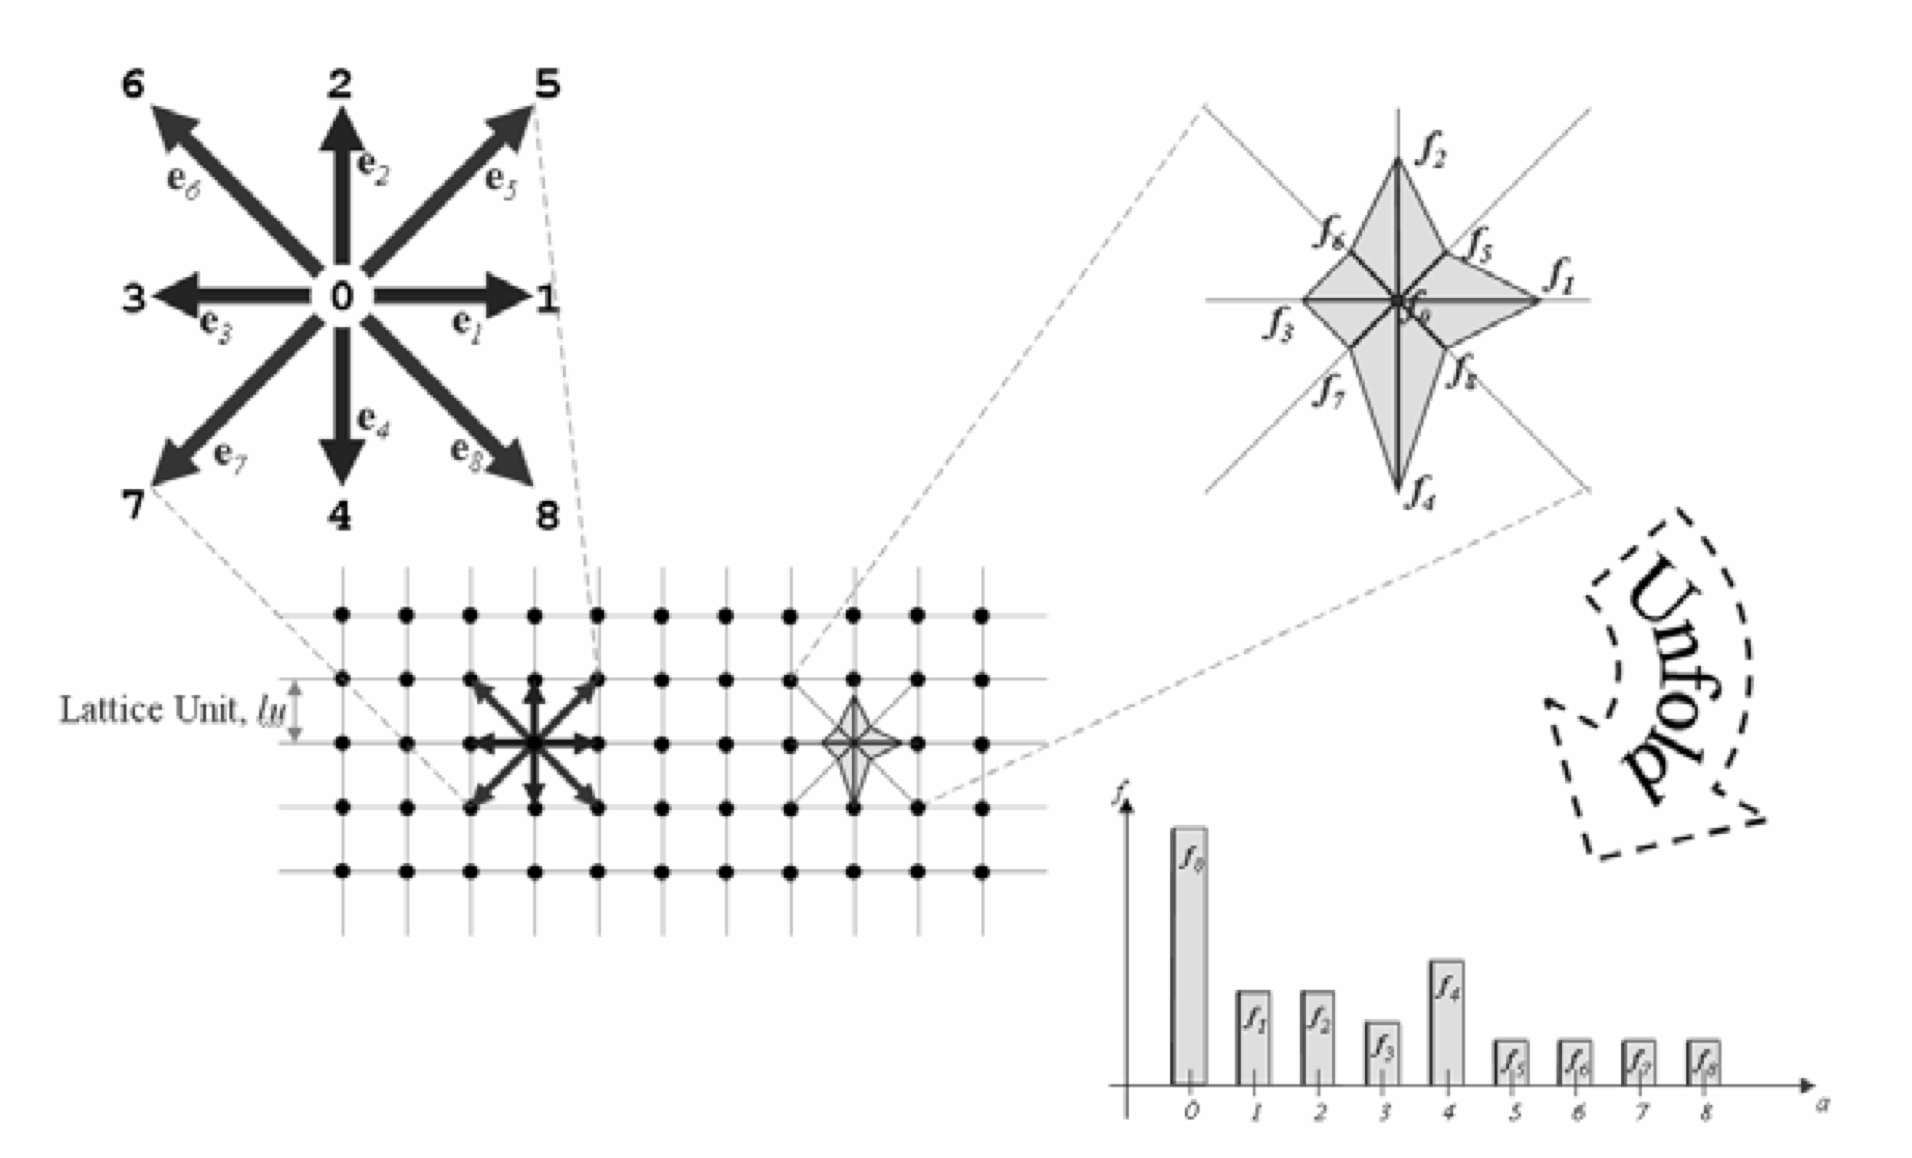
\includegraphics[width=0.8\linewidth]{latticeboltzmann.png}
	\captionof{figure}{Particle distributions of the Lattice Boltzmann Method. \tiny{Source: Michael C. Sukop}}
\end{posterbox}


\begin{posterbox}[name=geometry,span=4,column=2,row=0]{Generalized Geometry}
\begin{center}
\centering
\raisebox{-0.5\height}{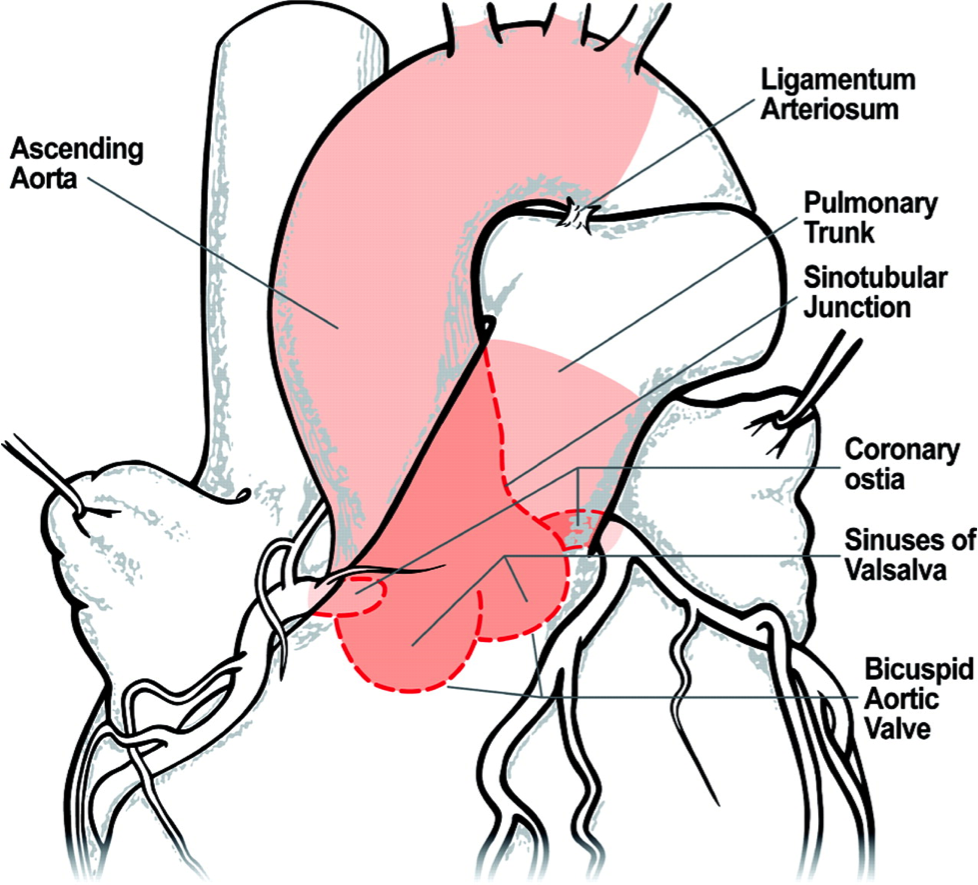
\includegraphics[width=3cm]{Aorta.png}}%
\raisebox{-0.5\height}{\hspace{0.5cm}$\longrightarrow$}%
\raisebox{-0.5\height}{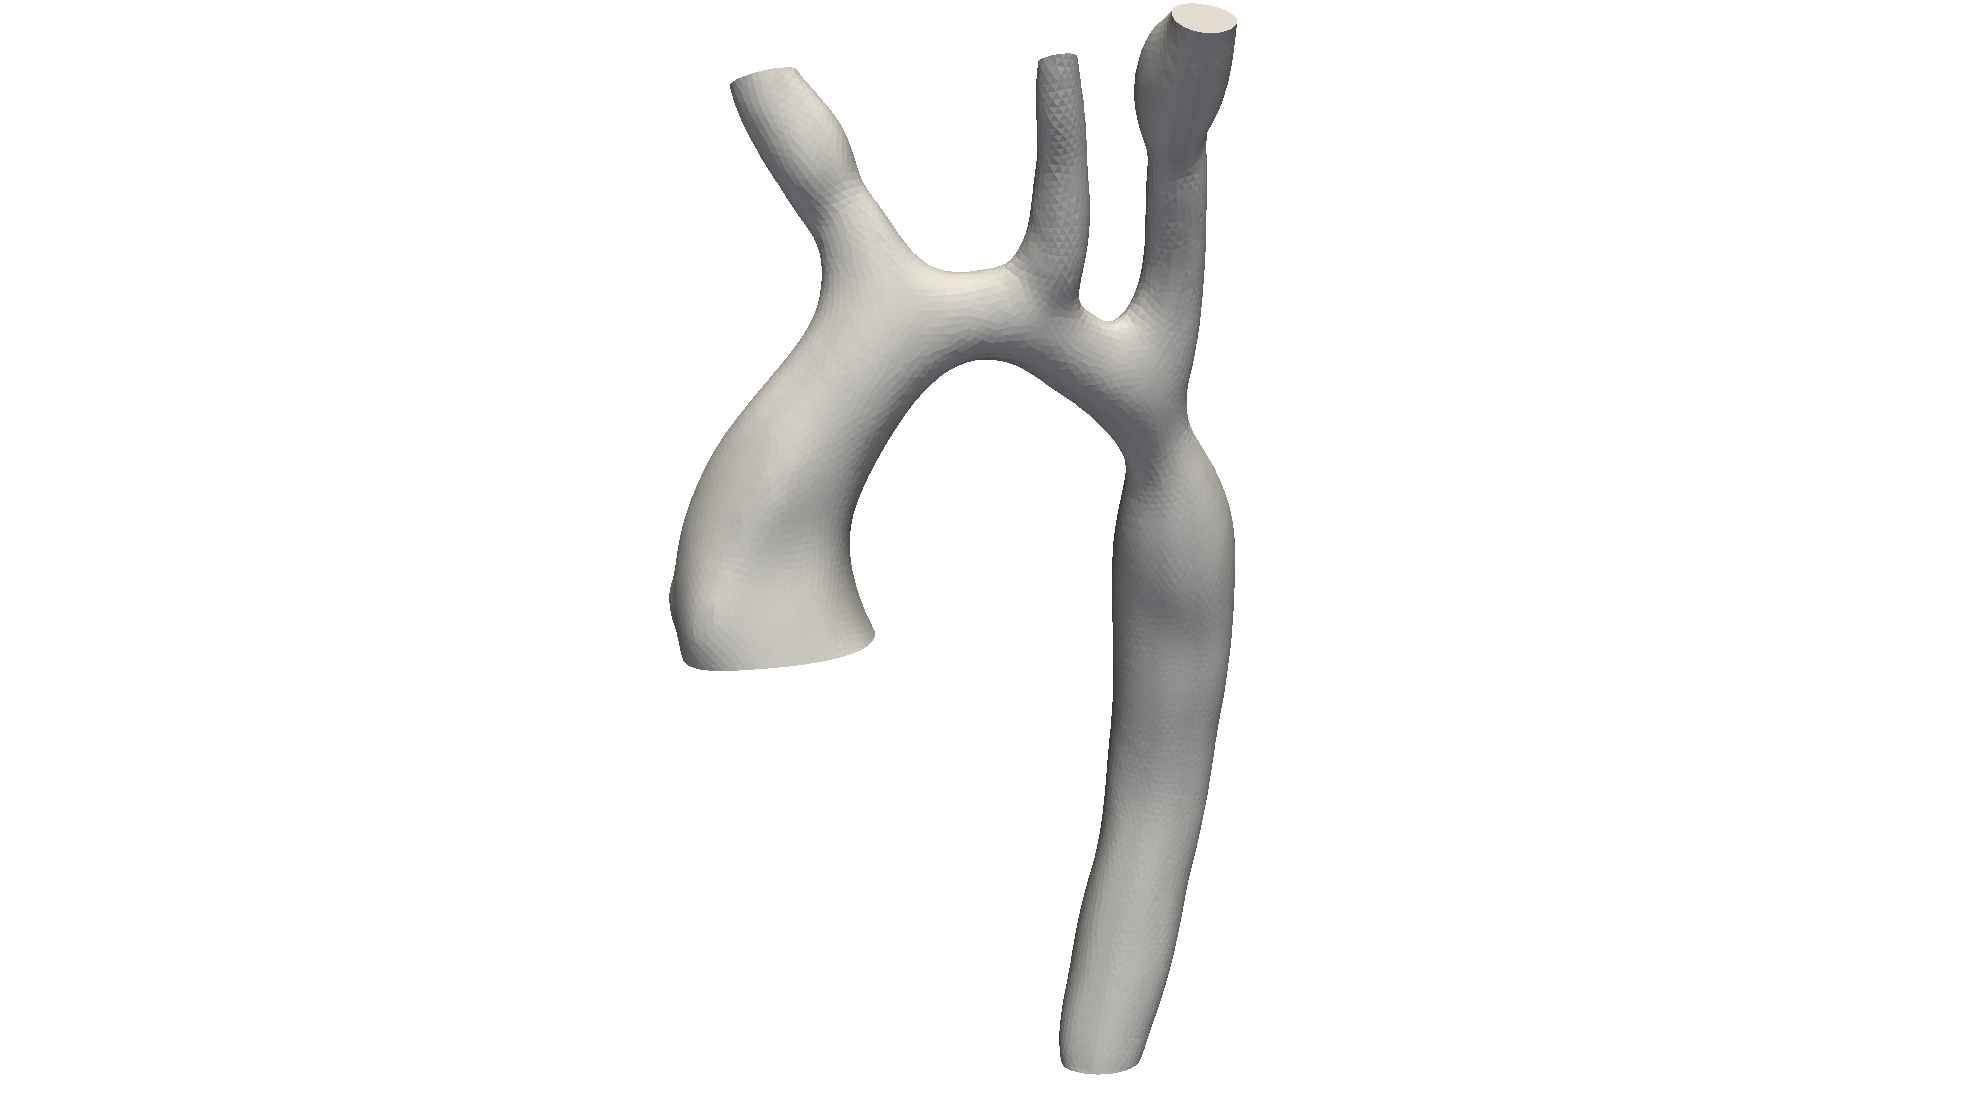
\includegraphics[trim = 13cm 0cm 15cm 0cm, clip=true,totalheight=3cm]{aorta3d.png}}%
\raisebox{-0.5\height}{\hspace{0.5cm}$\longrightarrow$\hspace{0.2cm}}%
\raisebox{-0.5\height}{\includegraphics[totalheight=2.25cm]{Arched_stenosis_3.png}}%
\raisebox{-0.5\height}{\hspace{0.5cm}$\longrightarrow$}%
\raisebox{-0.5\height}{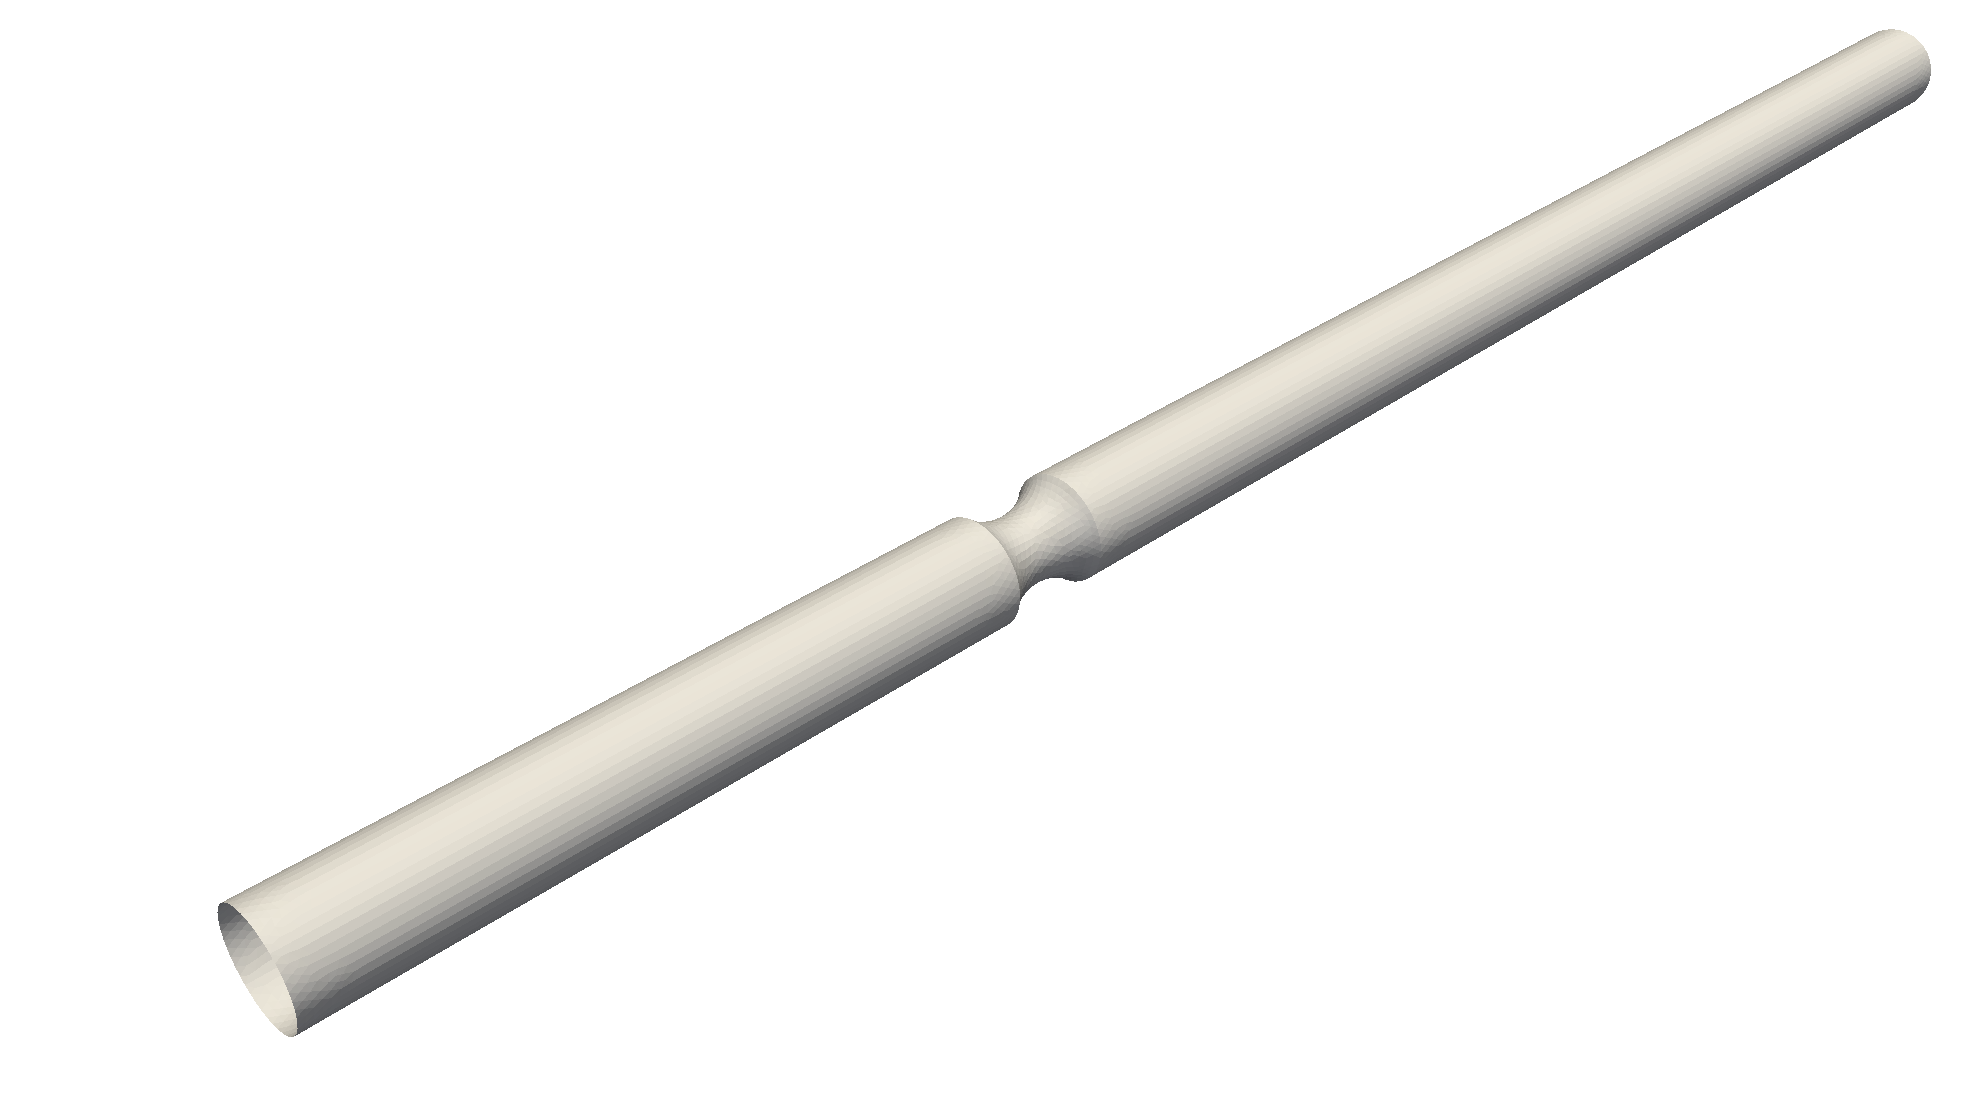
\includegraphics[height=2.25cm]{3d_stenosis_1.png}}%
\raisebox{-0.5\height}{\hspace{0.5cm}$\longrightarrow$\hspace{0.2cm}}%
\raisebox{-0.5\height}{
	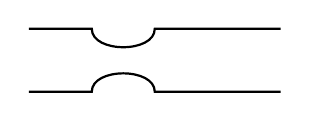
\begin{tikzpicture}[scale=0.4]
	\draw[thick] (0,0)--(2,0) to [out=90,in=90] (4,0)--(8,0);
	\draw[thick] (0,2)--(2,2) to [out=-90,in=-90] (4,2)--(8,2);
	\end{tikzpicture}
	}
\captionof{figure}{General Geometries of Simulation \tiny{(Left: America Heart Association, Second from Left: Aortic Segmentation from Fraunhofer MEVIS)}}
\end{center}
\end{posterbox}


\begin{posterbox}[name=equations,column=3,span=1, below=geometry]{Macroscopic Quantities}
From the distribution function $f$,  we can easily extract the typical macroscopic quantities which are used to analyze flow dynamics. Namely Density/Pressure and Velocity.
\beqs \rho\of{x,t} = \sum_{i=0}^8 f_i \of{x,t} \eeqs
\beqs \vec{u}\of{x,t} = \frac{1}{\rho}\sum_{i=0}^8 c_i \cdot f_i \cdot \vec{e_i} \eeqs 
\end{posterbox}


\begin{posterbox}[name=code,column=2,span=1, below=geometry, bottomaligned = equations]{Implementation}
\scriptsize
\begin{verbatim}
// Define Simulation Parameters
Conversion of Physical Units to Lattice Units

Initialize all active nodes to Equilibrium
Set fixed boundary conditions
for ( ti = 0; ti < tMax; ti++ ){
    Set time dependent boundary conditions:
        Inlet - Velocity Boundary 
        Outlet - Pressure Boundary 
    BounceBack Conditions on given nodes
	
    Collision Step (RHS of Equation 2)
    Steaming Step (LHS of Equation 2)
}	
\end{verbatim}
\end{posterbox}


\begin{posterbox}[name=results,column=2,span=4, below=equations]{Results in Two Dimensions}
\centering
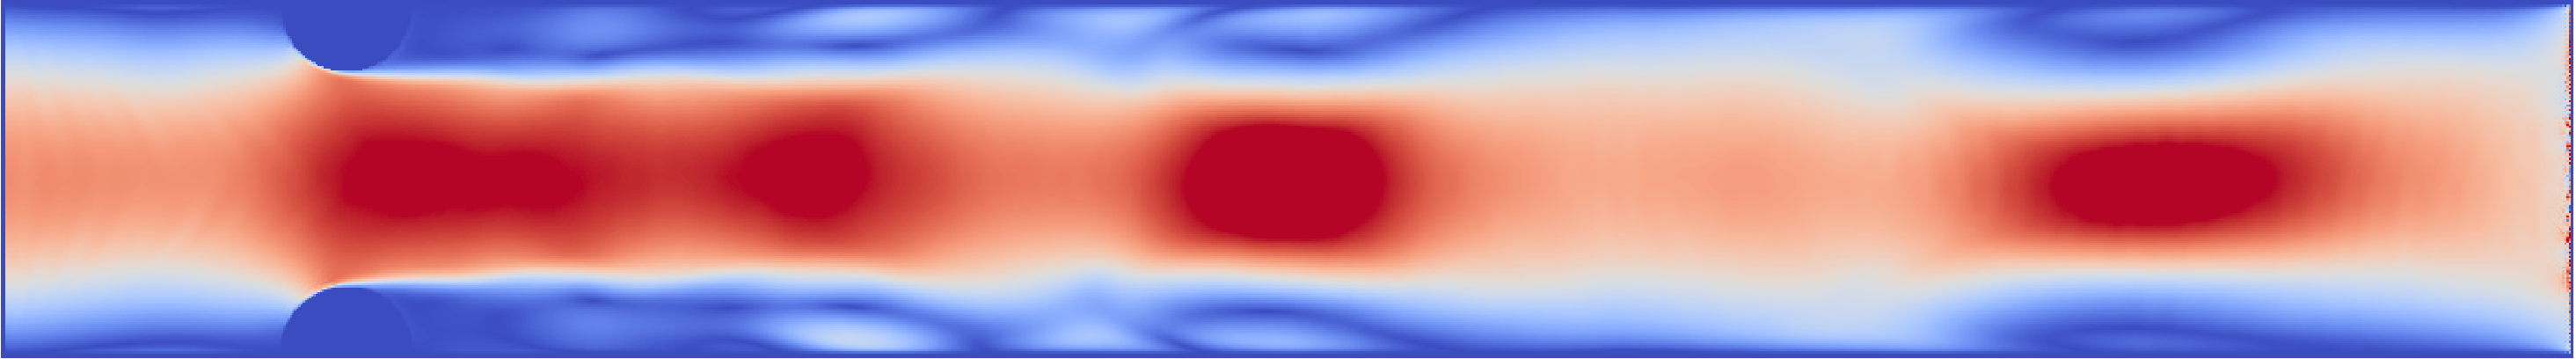
\includegraphics[height=1cm]{re875pres.png}\hspace{0.2cm}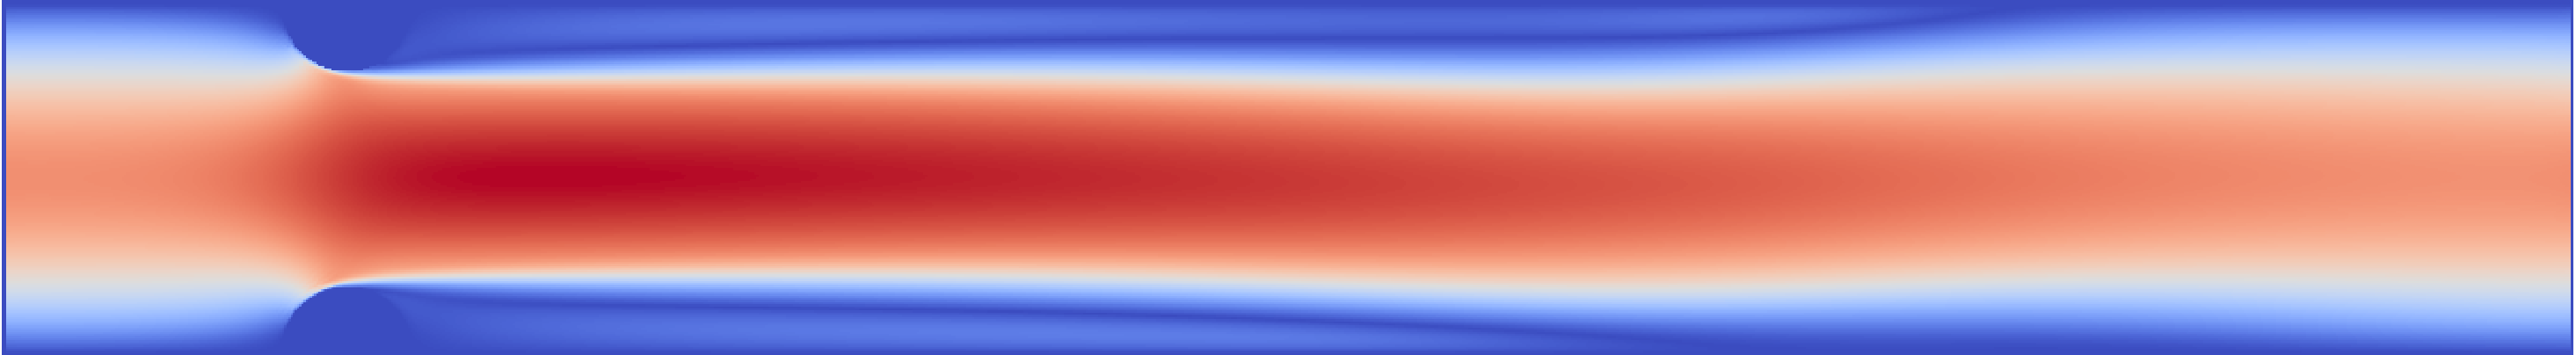
\includegraphics[height=1cm]{re875vel1.png}\hspace{0.2cm}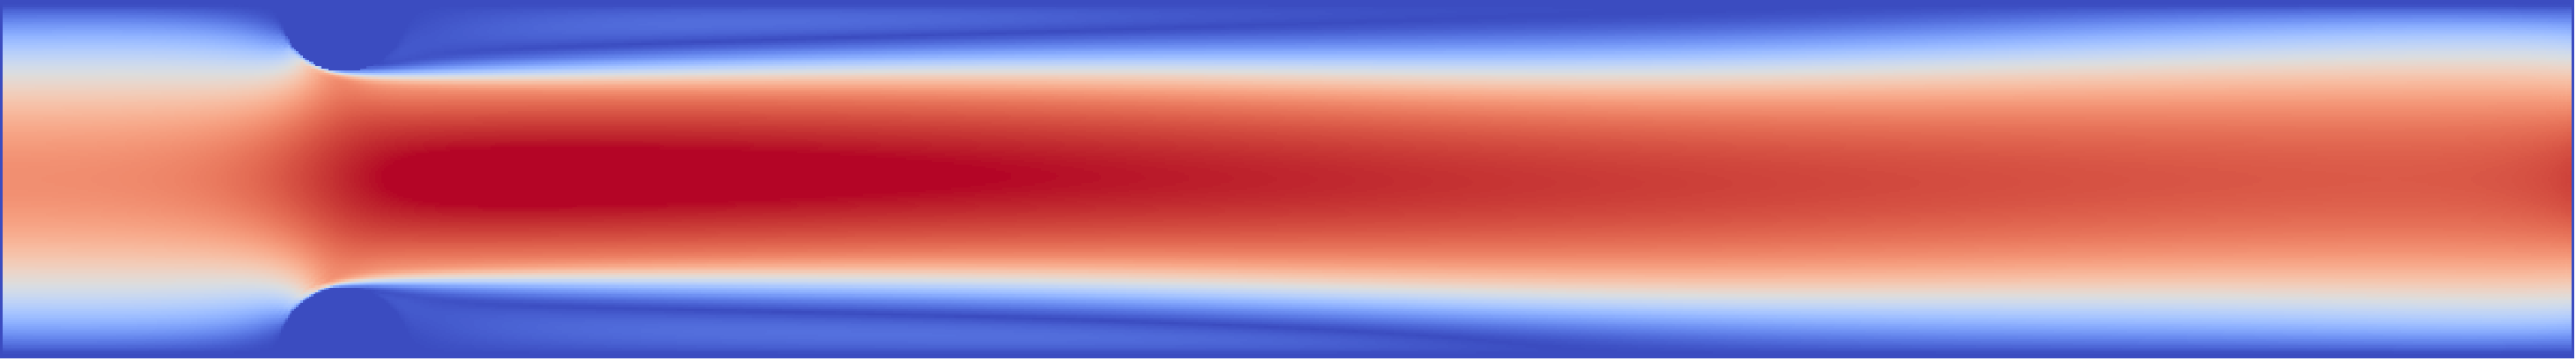
\includegraphics[height=1cm]{re875vel1_2.png}
\captionof{figure}{Flow patterns with Pressure(Left), Velocity with equivalent inflow and outflow(Middle), and Velocity with outflow $=1.2\cdot$inflow (Right) boundary conditions}
\vspace{0.1cm}
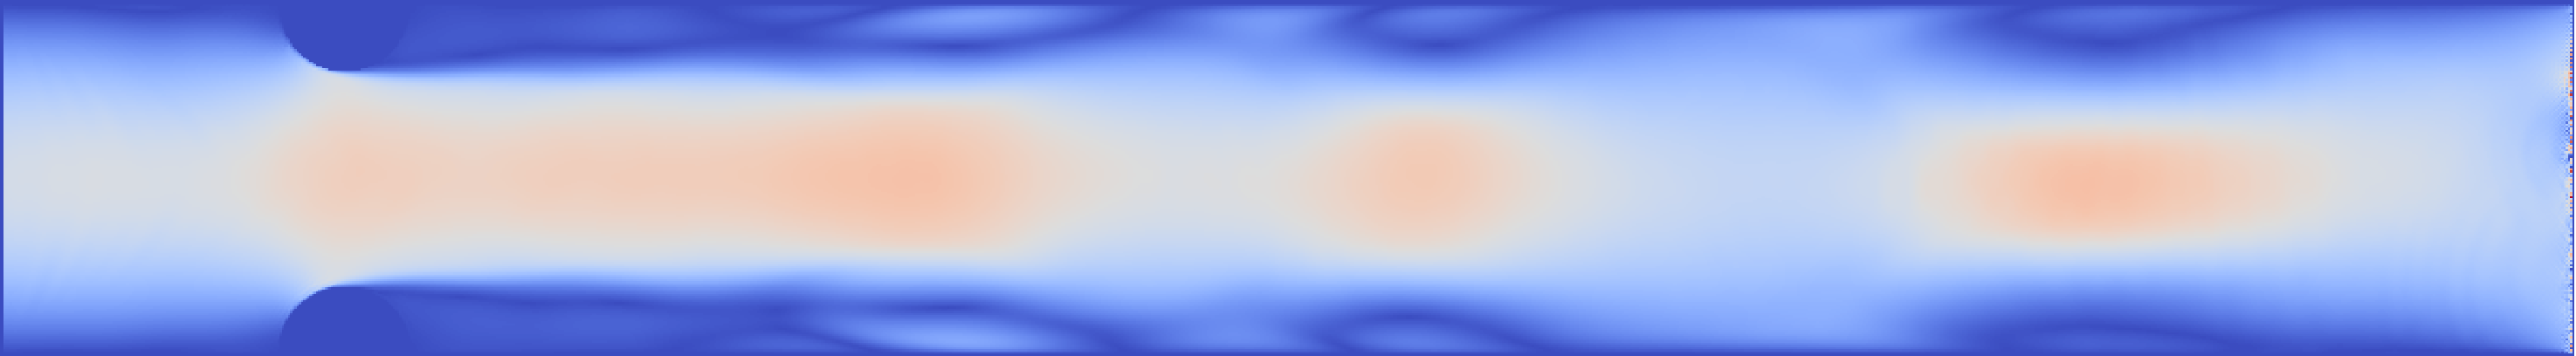
\includegraphics[height=1cm]{periodic_flow1.png}\hspace{1cm}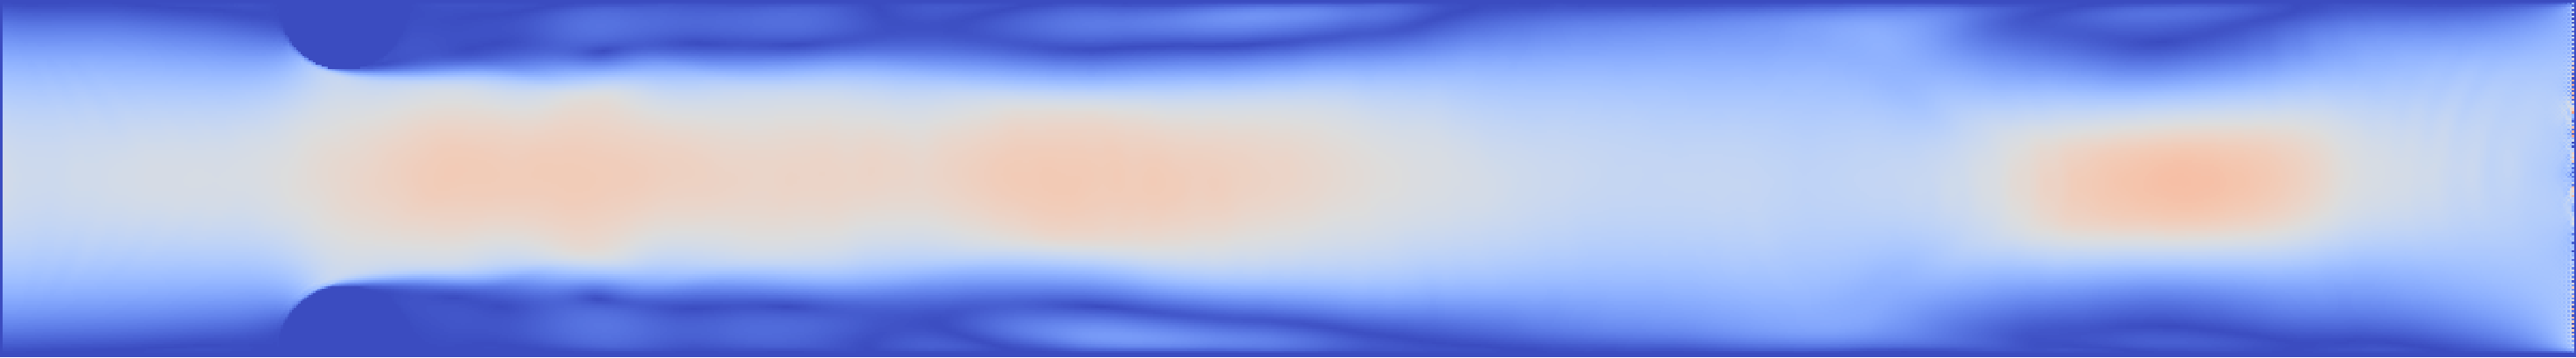
\includegraphics[height=1cm]{periodic_flow3.png}
\captionof{figure}{Simulation of Reynolds Number 1000 geometry with Pressure Boundary and Smagorinsky constants 0.2(Left) and 0.1(Right)}
\vspace{0.1cm}
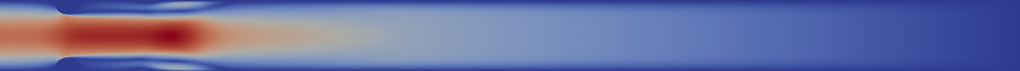
\includegraphics[height=1cm]{re-875_smago-02_vel0.png}
\captionof{figure}{Flow with a 0 velocity outflow profile and Smagorinski constant of 0.2, demonstrating stabilization of flow modeled with turbulent aspects in mind}
\end{posterbox}


\begin{posterbox}[name=figures,column=4,span=2, below=geometry, above=results]{Flow Through Idealized Stenosis using OpenLB}
\begin{center}
\includegraphics[height=4.5cm]{stenosis3d_maxsystole_5.png}
\end{center}
\end{posterbox}


\begin{posterbox}[name=future,column=2,span=2, below=results, bottomaligned=distribution]{Future Research}
Currently, the stability of the Zou-He\cite{zou_he:97} Pressure boundary conditions for a stenotic geometry, as well as the transition period of Reynolds Numbers where periodic flow is seen, are incomplete. As such more work needs to be done in the direction of classification of flow patterns with regards to Reynolds numbers as well as a thorough analysis to the boundary conditions needed in a geometry with increased outward velocity. Also as seen in the generalization of geometries above there exists a geometry, the arched stenosis, which has not yet been studied and may provide interesting results.
\end{posterbox}

% References, if required
\begin{posterbox}[
    name = ref,  % Name for alignment 
    column = 4, % Last column 
    span = 2,
    below = results, % Alignment
    bottomaligned = distribution % Alignment 
    ]{References}
    \renewcommand{\section}[2]{} % Get rid of the default "References" section title
    \nocite{*} % Insert publications even if they are not cited in the poster
    \bibliography{Bibliography}
    \bibliographystyle{abbrv}
\end{posterbox}
\end{poster}
\end{document}